\chapter{Esecuzione}
\label{ch:results}
Qui vengono confrontati i due algoritmi REPTree e RIPPER/JRip. Entrambi hanno sfruttato una \textit{10-fold cross validation}.

\section{Risultati su \texttt{German Credit}}

\normalsize L'esecuzione ha coinvolto 900 istanze di training e 100 istanze di testing ad ogni iterazione del CV.

\begin{mdframed}[frametitle=Esecuzione NaiveBayesSimple]
	\footnotesize\verbatiminput{results/nb/german_credit.nb}
\end{mdframed}


\begin{mdframed}[frametitle=Esecuzione REPTree]
	\footnotesize\verbatiminput{results/reptree/german_credit.reptree}
\end{mdframed}


\begin{sidewaysfigure}
	\thisfloatpagestyle{empty}
	\makebox[\textwidth]{
\includegraphics[width=1.4\textwidth, height=.4\textheight]{results/reptree/gc.pdf}}
	\caption{Modello di REPTree}
\end{sidewaysfigure}

\pagebreak

\begin{mdframed}[frametitle=Esecuzione JRip]
	\footnotesize\verbatiminput{results/jrip/german_credit.jrip}
\end{mdframed}


\noindent
\normalsize Regole:
\footnotesize\input{results/jrip/german_credit.list.rules}

\pagebreak

\section{Risultati su \texttt{Hepatitis}}

\normalsize L'esecuzione ha coinvolto 139 istanze di training e 16 istanze di testing ad ogni iterazione del CV.

\begin{mdframed}[frametitle=Esecuzione NaiveBayesSimple]
	\footnotesize\verbatiminput{results/nb/hepatitis.nb}
\end{mdframed}


\begin{mdframed}[frametitle=Esecuzione REPTree]
	\footnotesize\verbatiminput{results/reptree/hepatitis.reptree}
\end{mdframed}


\begin{figure}[htb]
	\makebox[\textwidth]{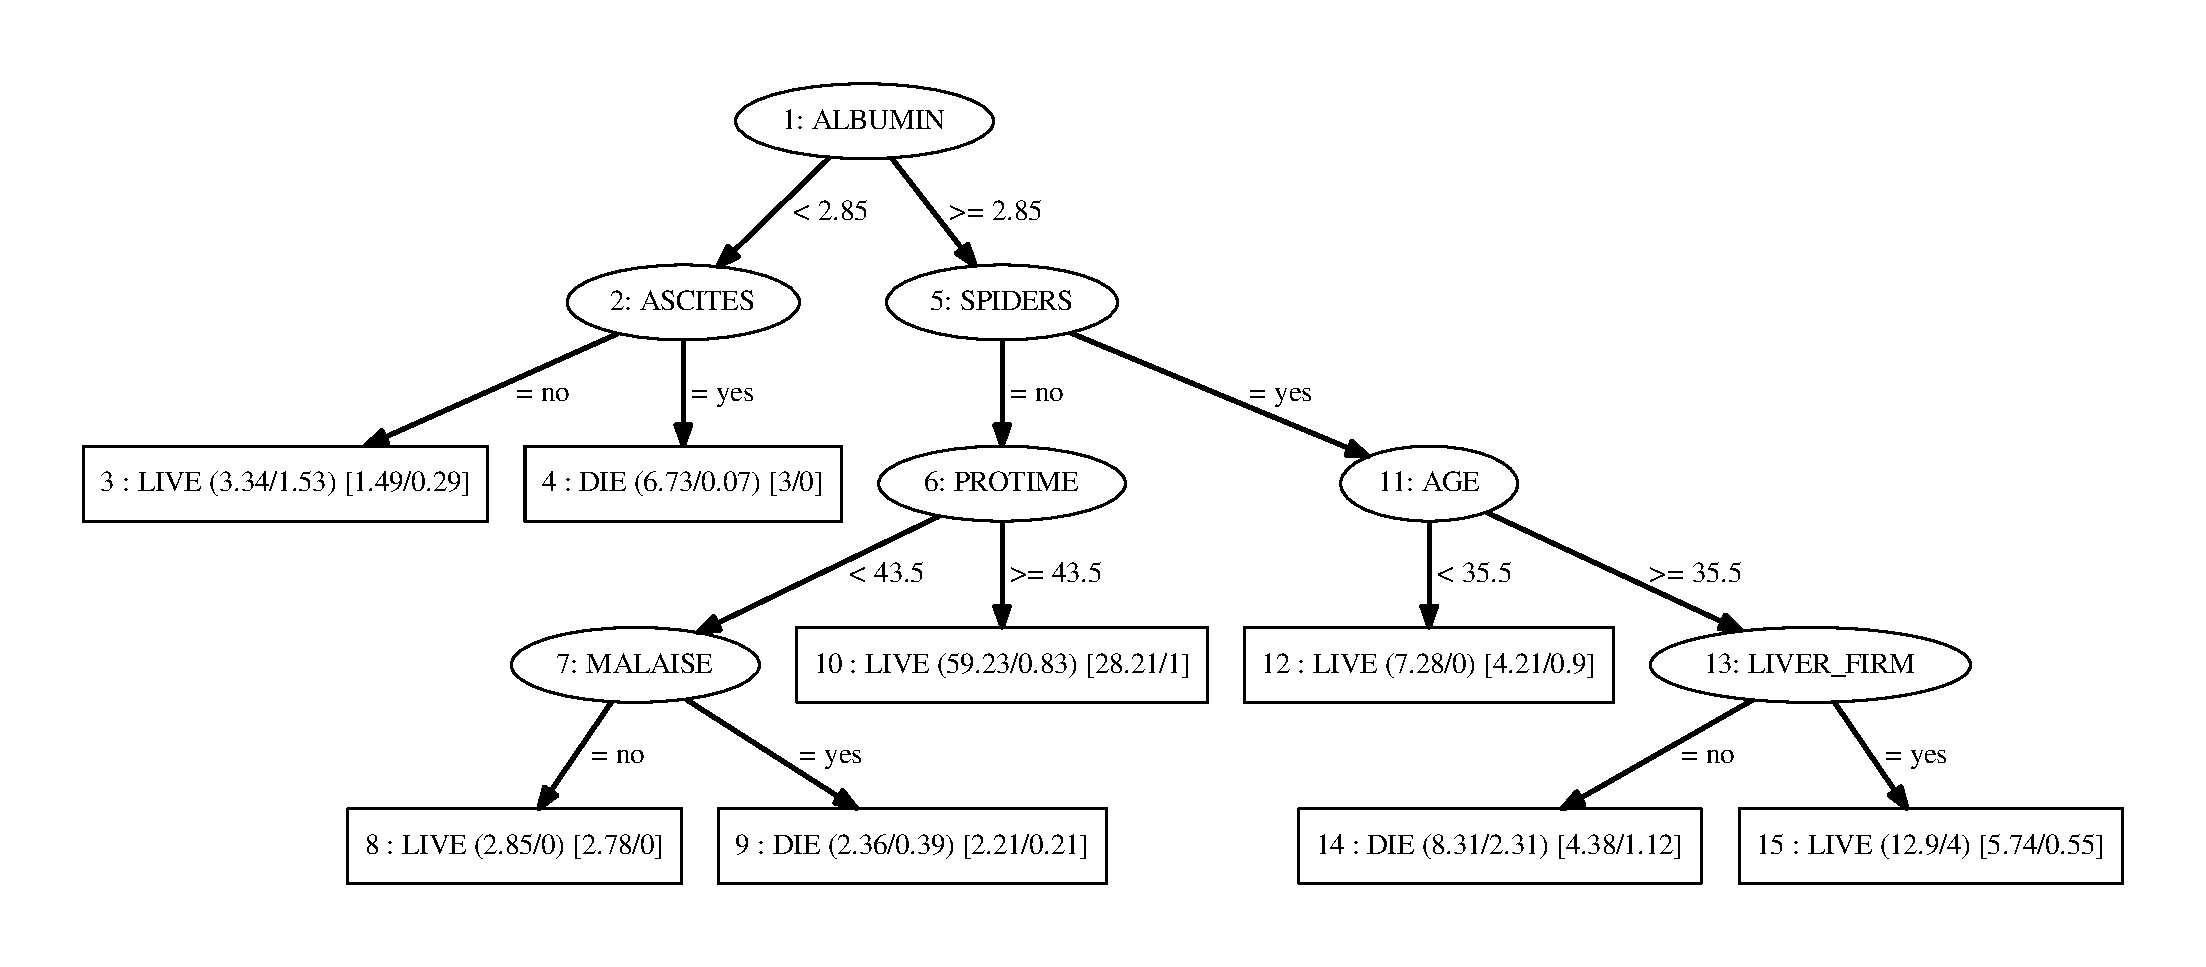
\includegraphics[width=1.55\textwidth]{results/reptree/hepatitis.pdf}}
	\caption{Modello di REPTree}
\end{figure}

\begin{mdframed}[frametitle=Esecuzione JRip]
	\footnotesize\verbatiminput{results/jrip/hepatitis.jrip}
\end{mdframed}


\noindent
\normalsize Regole:
\footnotesize\input{results/jrip/hepatitis.list.rules}

\pagebreak

\section{Risultati su \texttt{Vehicle Silhouettes}}

\normalsize L'esecuzione ha coinvolto 761 istanze di training e 85 istanze di testing ad ogni iterazione del CV.

\begin{mdframed}[frametitle=Esecuzione NaiveBayesSimple]
	\footnotesize\verbatiminput{results/nb/vehicle.nb}
\end{mdframed}


\begin{mdframed}[frametitle=Esecuzione REPTree]
	\scriptsize\verbatiminput{results/reptree/vehicle.reptree}
\end{mdframed}


\begin{figure}[htb]
	\makebox[\textwidth]{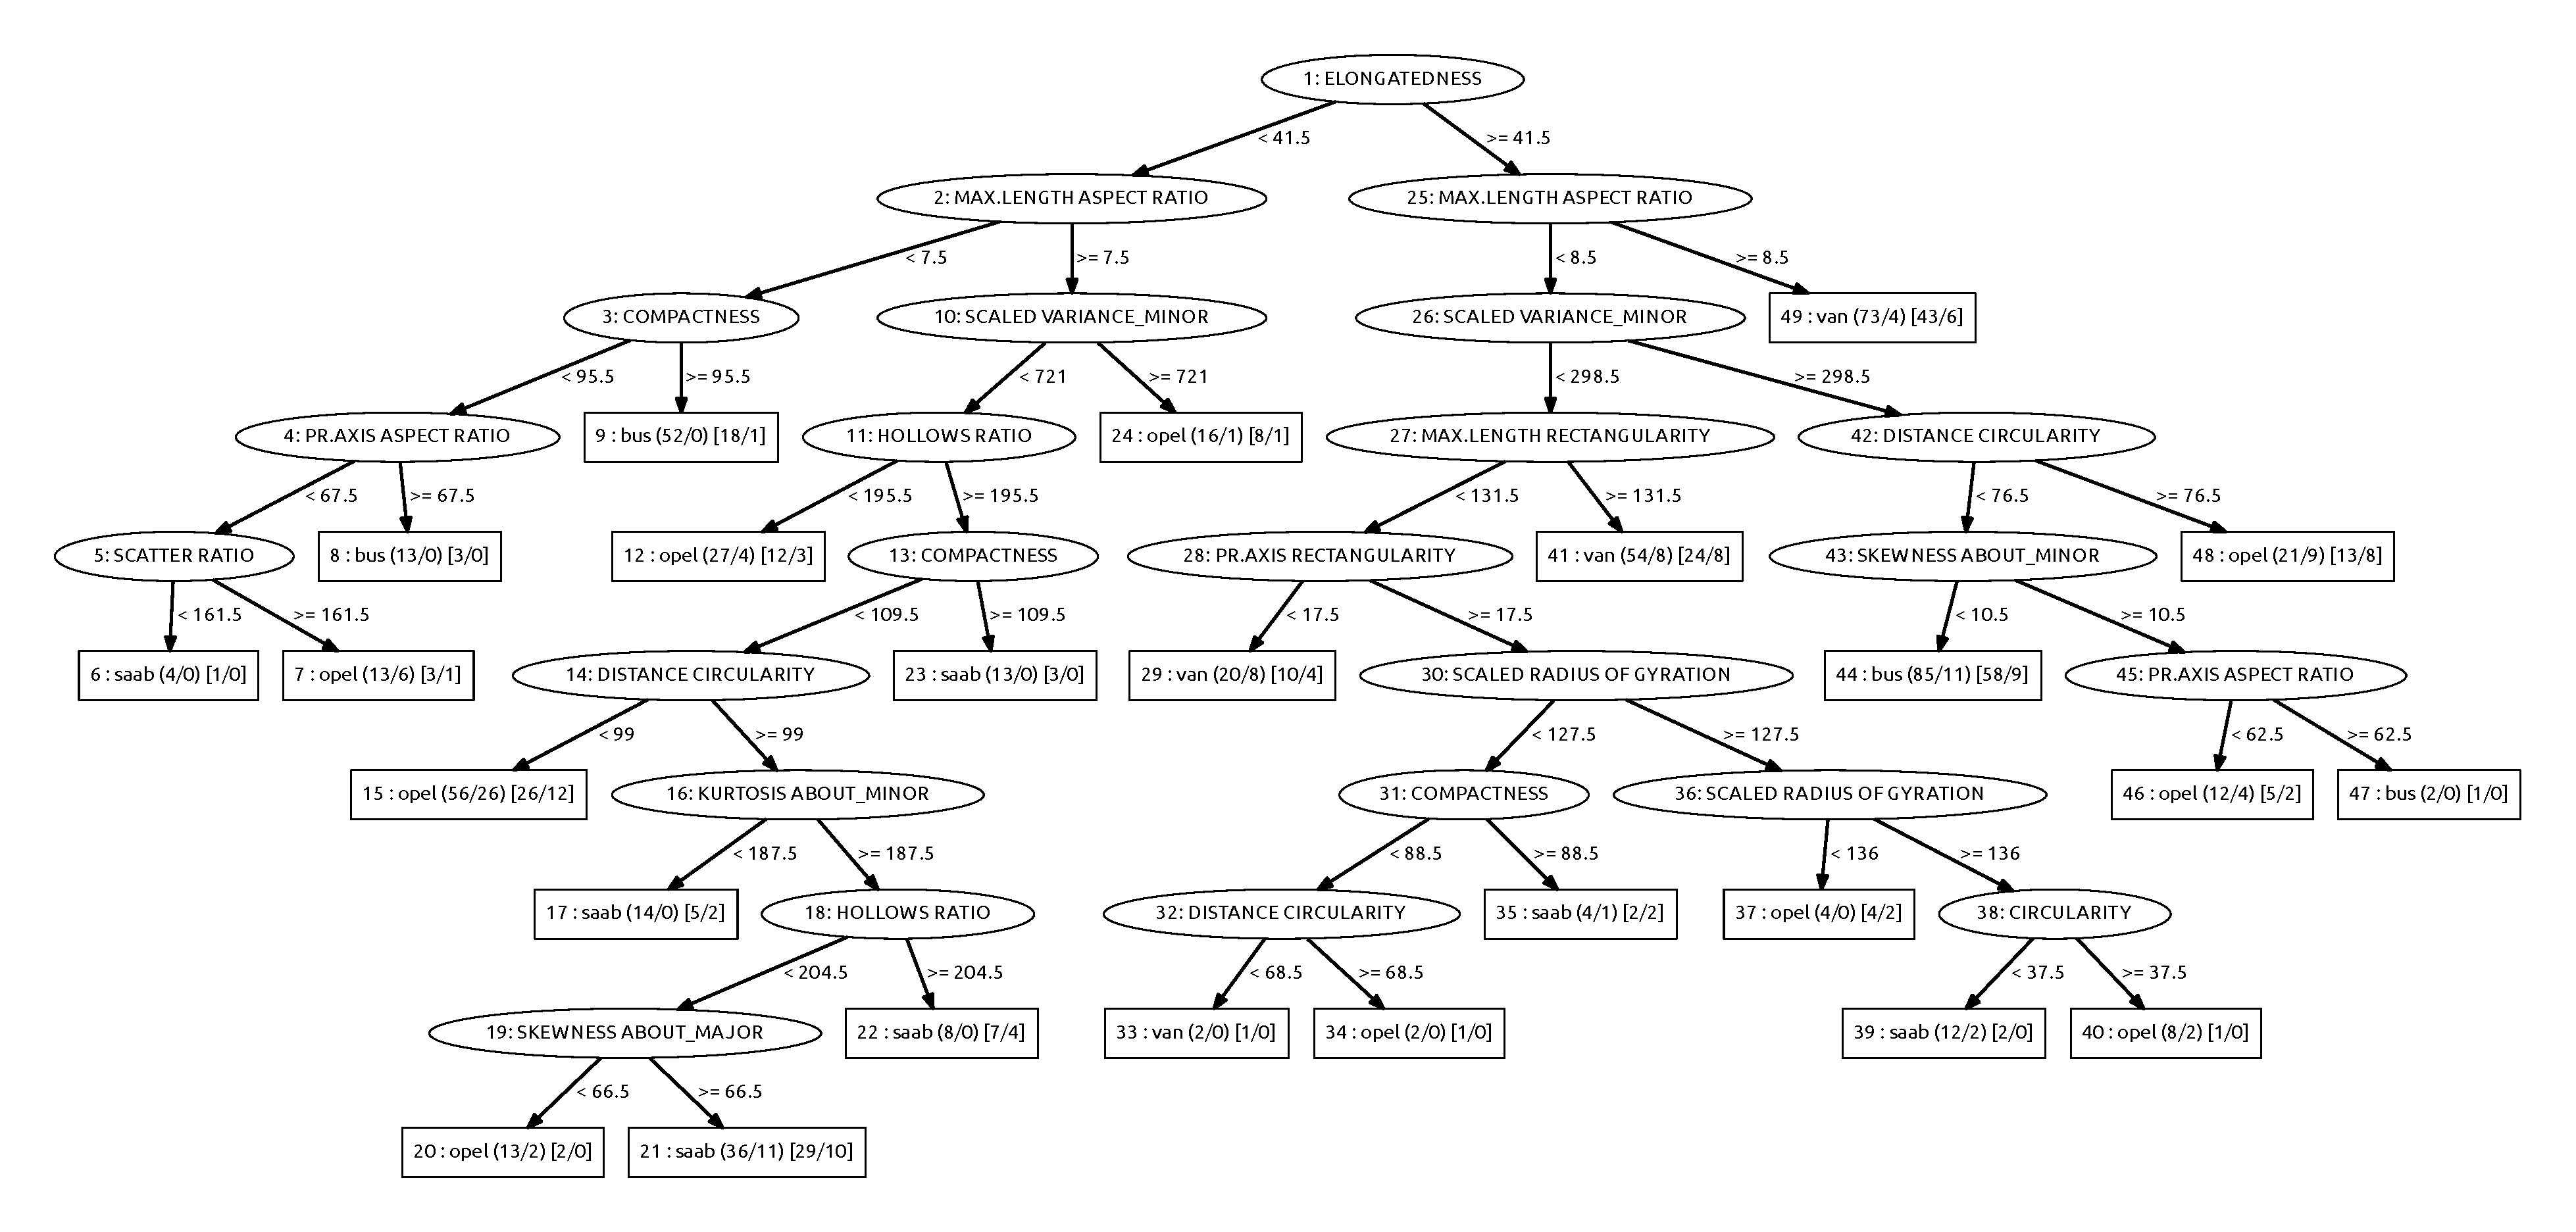
\includegraphics[width=1.55\textwidth]{results/reptree/vehicle.pdf}}
	\caption{Modello di REPTree}
\end{figure}

\begin{mdframed}[frametitle=Esecuzione JRip]
	\scriptsize\verbatiminput{results/jrip/vehicle.jrip}
\end{mdframed}


\noindent
\normalsize Regole:
\scriptsize\input{results/jrip/vehicle.list.rules}

\pagebreak

\section{Risultati su \texttt{Wisconsin Breast Cancer}}

\normalsize L'esecuzione ha coinvolto 629 istanze di training e 70 istanze di testing per ogni fold.


\begin{mdframed}[frametitle=Esecuzione NaiveBayesSimple]
	\footnotesize\verbatiminput{results/nb/wbc.nb}
\end{mdframed}

\begin{mdframed}[frametitle=Esecuzione REPTree]
	\footnotesize\verbatiminput{results/reptree/wisconsin_breast_cancer.reptree}
\end{mdframed}


\begin{figure}[htb]
	\makebox[\textwidth]{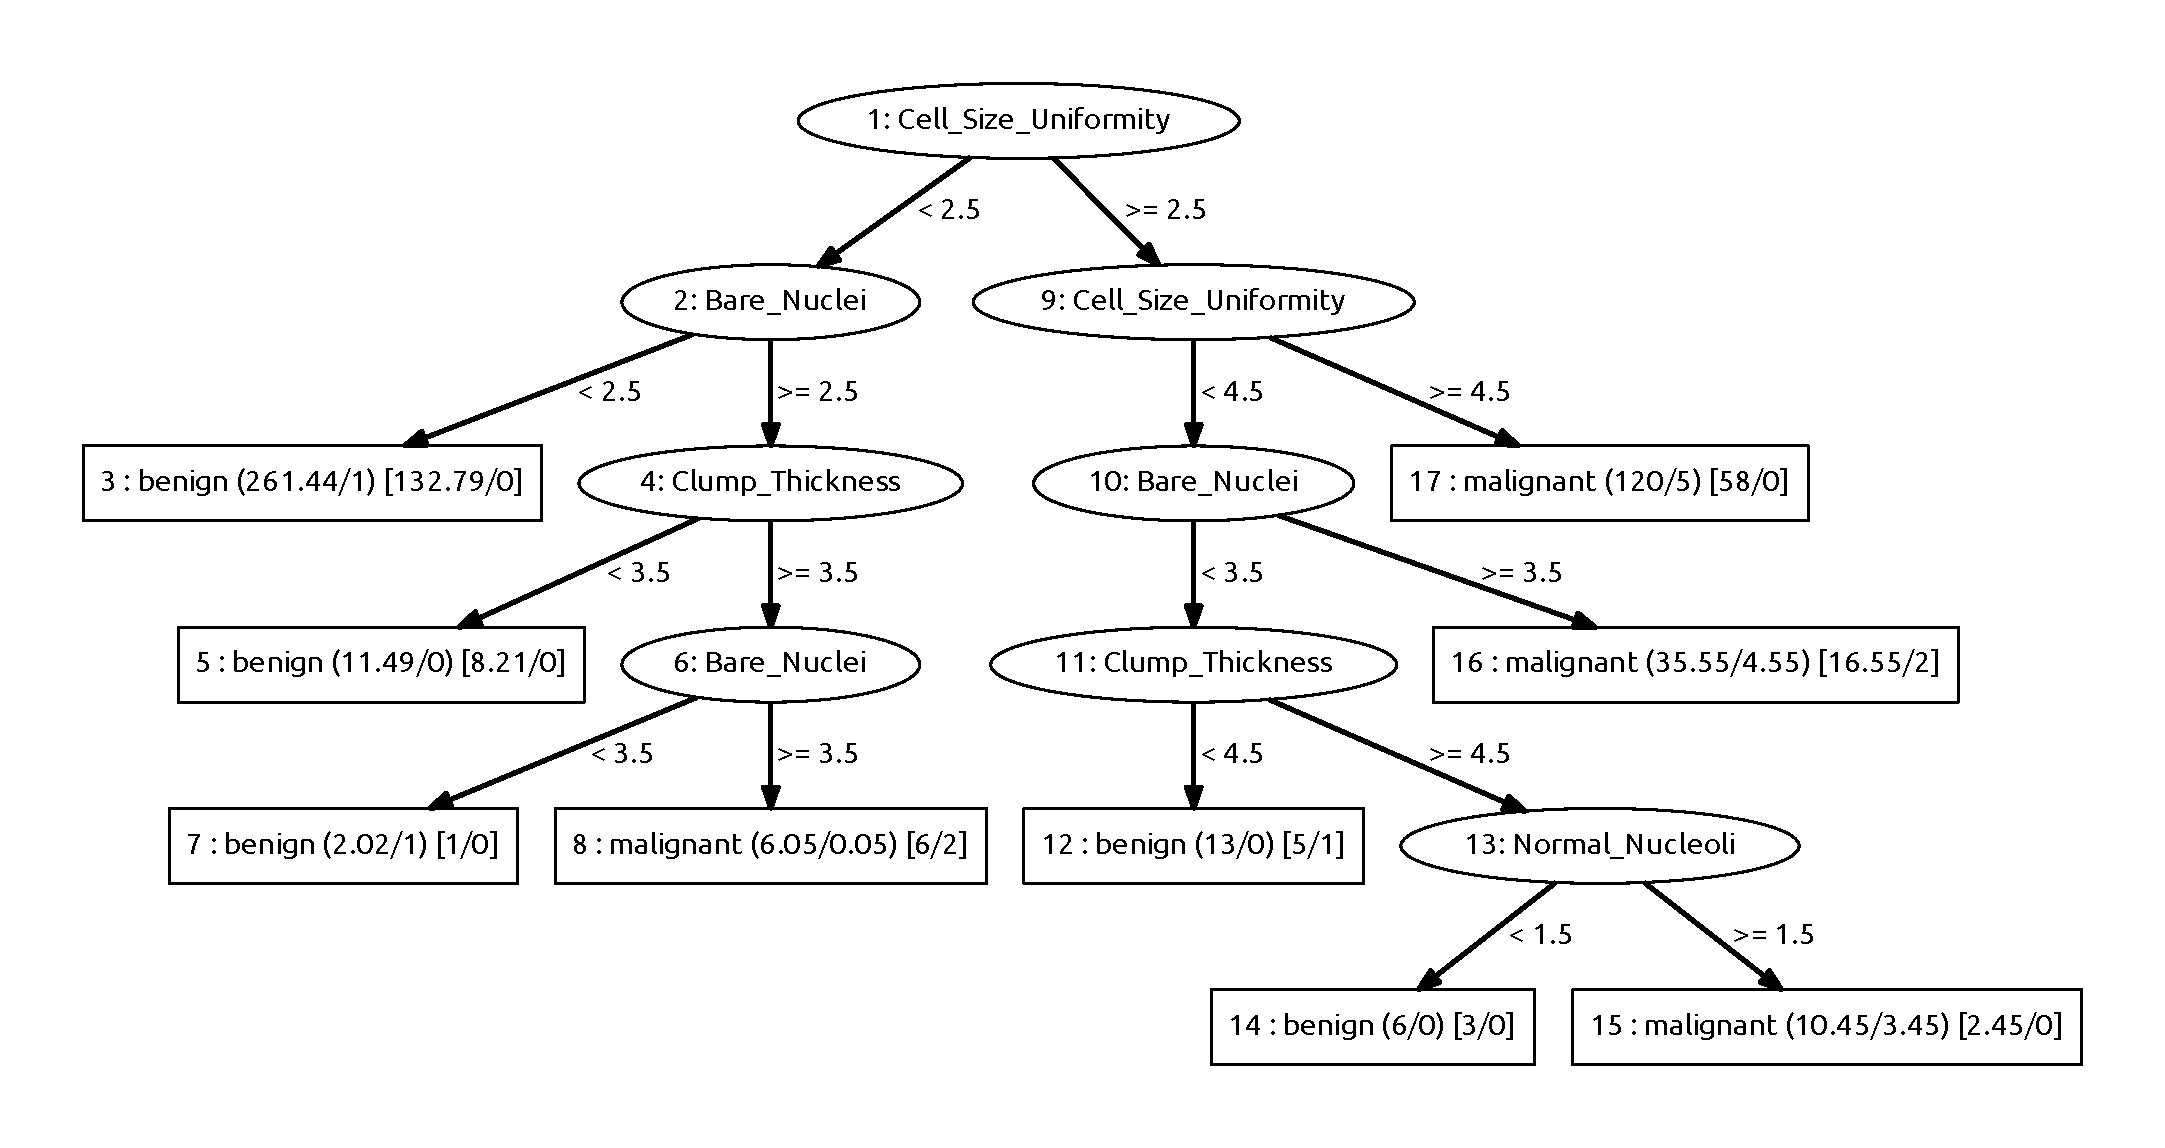
\includegraphics[width=1.55\textwidth]{results/reptree/wisconsin_breast_cancer.pdf}}
	\caption{Modello di REPTree}
\end{figure}

\begin{mdframed}[frametitle=Esecuzione JRip]
	\footnotesize\verbatiminput{results/jrip/wisconsin_breast_cancer.jrip}
\end{mdframed}


\noindent
\normalsize Regole:
\footnotesize\input{results/jrip/wisconsin_breast_cancer.list.rules}